\documentclass[t]{beamer}

%\documentclass[handout, t]{beamer}
\setbeamertemplate{navigation symbols}{}
\usepackage{pstricks}
\usepackage{mathtools}
\usepackage{amsfonts}
\usepackage{mathrsfs}
\usepackage{amsmath}
\usepackage{physics}
\setbeamertemplate{navigation symbols}{}
\usepackage{bm}
\usepackage[UTF8]{ctex}
\usetheme{AnnArbor}
\usefonttheme{serif}
\useinnertheme{rounded}
\usecolortheme{beaver}
\setbeamertemplate{blocks}[rounded][shadow=true]

\newcommand{\dif}{{\;\rm d}}
\usepackage{graphicx}
\usepackage{pgf}
\usepackage{tikz}
\usetikzlibrary{arrows, decorations.pathmorphing, backgrounds, positioning, fit, petri, automata}
\tikzset{>=stealth}

\usepackage{setspace}
\setmainfont{Times New Roman}
\setCJKmainfont{Microsoft YaHei}
% \setCJKmainfont{苹方}   % 使用苹果MAC系统,请使用这个选项,并将上面的命令用%注释掉

\hypersetup{pdfpagemode=FullScreen}
\renewcommand{\Pr}{\mathbb{P}}
\usepackage{blkarray}


\setbeamercolor{block title}{bg=red!10!white}
\setbeamercolor{block body}{bg=gray!10!white}

\usepackage{multicol}
\newcommand{\E}{\mathbb{E}}
\newcommand{\EP}{\mathbb{E}^{\mathbb{P}}}
\newcommand{\EQ}{\mathbb{E}^{\mathbb{Q}}}
\newcommand{\Var}{{\rm Var}}
\newcommand{\Cov}{{\rm Cov}}


\begin{document}
\fontsize{11}{18}\selectfont


\CTEXindent



  \title{第四章~~随机积分概论}
\author{金融数学}
\date{中国人民大学出版社}
  \begin{frame}
    \maketitle
  \end{frame}



\begin{frame}{本章内容}


    \tableofcontents


\end{frame}


\section{普通积分回顾}
\begin{frame}{普通积分}
对于一个普通确定性积分(deterministic integral),可以通过对确定性的函数进行相关的运算操作,进而进行求解。比如:
\begin{equation*}
R(T)=\int^T_0 g(t)\dif t 
\end{equation*}
此处的积分求解,可以使用离散化函数定义域$[0,T]$的方式,通过对求和取极限的方式得到。以上式为例,我们对$[0,T]$进行划分,可以得到该时间段的一个分划(partition),即:
\[0=t_0< t_1< \cdots< t_n=T \]
\end{frame}


\begin{frame}{普通积分的黎曼和}
据此可以得到关于这个确定性积分的近似计算方法,称之为黎曼和(Riemann sum),具体形式如下:
\[R_1= \sum^{n-1}_{i=0}g(t_{i})(t_{i+1}-t_{i}) \]

我们也可以通过选取$[t_i,t_{i+1}]$时间段中的任何一点的$g(\xi_i)$取值作为矩形的高度,即:
\[R_2= \sum^{n-1}_{i=0}g\left(\xi_i\right)(t_{i+1}-t_{i}), \quad \xi_i\in[t_i,t_{i+1}]\]
\end{frame}


\begin{frame}{黎曼和的图形展示}
\begin{multicols}{2}
	\centering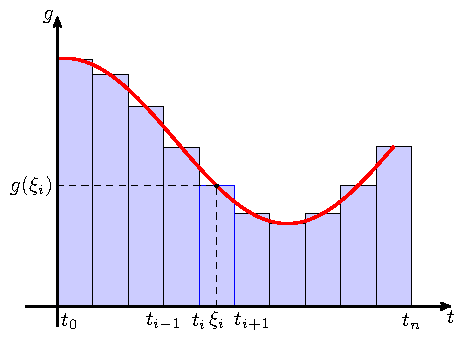
\includegraphics[scale=0.95]{fig/riemann-sum.pdf}

\[\begin{split}
R(T)&=\int^T_0 g(t)\dif t \\
R_1&= \sum^{n-1}_{i=0}g(t_{i})(t_{i+1}-t_{i})\\
R_2&= \sum^{n-1}_{i=0}g\left(\xi_i\right)(t_{i+1}-t_{i})\\
\xi_i&\in[t_i,t_{i+1}]
\end{split}\]
\end{multicols}
\end{frame}

\begin{frame}{黎曼积分}
这种基于对定义域切割所进行的积分求解方法,称为黎曼积分(Riemann integral)。
不太严格地来说,黎曼积分就是当分割越来越“精细”的时候,黎曼和趋向的极限。

记对时间段$[0,T]$的划分当中,最长的时间段为$\|\Pi\|$,即:
$\|\Pi\|=\max(t_{i+1}-t_{i}),\quad i=0,1,2,\ldots,n-1 $,于是有:
\[R(T)=\int^T_0 g(t)\dif t=\lim_{\substack{\|\Pi\|\to 0 \\ n\to\infty}}\sum^{n-1}_{i=0}g\left(\xi_i\right)(t_{i+1}-t_{i}) \]

对于光滑函数$g(t)$而言,其二次变差为零,相应的每个小区间中$g(\xi_i)$取值对最终的积分结果没有影响。
\end{frame}


\begin{frame}{黎曼-斯蒂尔切斯积分}
对于光滑函数$f(t)$和$g(t)$,以下积分称为黎曼-斯蒂尔切斯积分(Riemann-Stieltjes integral),简称RS积分:
\begin{equation*}
RS(T)=\int^T_0 g(t)\dif f(t) 
\end{equation*}

与黎曼积分类似,RS积分也有类似的黎曼和形式的表达方式,也就是黎曼-斯蒂尔切斯和(Riemann-Stieltjes sum)。
\begin{equation*}
\begin{split}
RS_1&= \sum^{n-1}_{i=0}g(t_{i})\big[f(t_{i+1})-f(t_{i})\big]\\
RS_2&= \sum^{n-1}_{i=0}g(\xi_i)\big[f(t_{i+1})-f(t_{i})\big],\qquad  \xi_i\in[t_i,t_{i+1}]
\end{split}
\end{equation*}
\end{frame}

\begin{frame}{黎曼-斯蒂尔切斯积分(cont.)}
同样,当划分的区间数$n\to\infty$时:
\[RS(T)=\int^T_0 g(t)\dif f(t)=\lim_{\substack{\|\Pi\|\to 0 \\ n\to\infty}}\sum^{n-1}_{i=0}g\left(\xi_i\right)\big[f(t_{i+1})-f(t_{i})\big] \]

由于光滑函数$f(t)$和$g(t)$的二次变差均为零,对应的每个小区间中$g(\xi_i)$取值对最终的积分结果没有影响。
\end{frame}

\section{随机积分的构造}
\begin{frame}{随机积分的形式}
随机积分的一般形式如下:
\begin{equation*}
I(T)=\int^T_0 g(t)\dif W(t)
\end{equation*}
其中:$W(t)$是$\mathcal{F}(t)$可测的布朗运动,并且$W(t)\sim \mathcal{N}(0,t)$;$g(t)$是一个$\mathcal{F}(t)$可测的随机过程;上述积分对应的概率空间为$(\Omega,\mathcal{F},\Pr)$。

\begin{block}{注意:}
布朗运动处处连续且处处不可微,我们无法像普通积分那样,将$\dif W(t)$写成$W'(t)\dif t$。所以普通的积分方法对这里的随机积分是无效的。
\end{block}
\end{frame}

\begin{frame}{随机积分$I(T)=\int^T_0 g(t)\dif W(t)$}
对$[0,T]$时间段进行剖分,假设$\{t_0,t_1,\ldots,t_n\}$是对该时间段的一个分划(partition),即:
$0=t_0< t_1< \cdots< t_n=T $

假设$g(t)$在每个子区间$[t_i,t_{i+1}),\; i=1,2,\ldots,n-1$内均是常数,分别记作$g(t_i)$。这样的过程$\{g(t_i)\}$称作简单过程(simple process)。
\end{frame}

\begin{frame}{随机积分$I(T)=\int^T_0 g(t)\dif W(t)$ (cont.)}
将$W(t)$想象成时刻$t$每股股票的价格;$g(t_i)$想象成子区间$[t_i,t_{i+1})$内持有的股票数量,则股票在$t$时刻的总价值$I(t)$分别为:
\[\normalsize I(t)= \begin{cases}
g(t_0)[W(t)-W(t_0)]=g(0)  W(t)    & t\in[t_0,t_1]\\
g(0)W(t_1)+g(t_1)[W(t)-W(t_1)]     & t\in[t_1,t_2]\\
g(0)W(t_1)+g(t_1)[W(t_2)-W(t_1)]+g(t_2)[W(t)-W(t_2)]     & t\in[t_2,t_3]\\
     \cdots\cdots\cdots\cdots\cdots &\cdots
\end{cases} \]
因此:若$t\in[t_k,t_{k+1}]$,则有:
\begin{equation*}
I(t)=\sum^{k-1}_{i=0}g(t_i)[W(t_{i+1})-W(t_{i})]+g(t_k)[W(t)-W(t_k)]
\end{equation*}
\end{frame}

\begin{frame}{随机积分$I(T)=\int^T_0 g(t)\dif W(t)$ (cont.)}
\begin{block}{注意:}
\begin{equation*}
I(t)=\sum^{k-1}_{i=0}g(t_i)[W(t_{i+1})-W(t_{i})]+g(t_k)[W(t)-W(t_k)]
\end{equation*}
其中的$g(t_i)$是基于时间区间$[t_i,t_{i+1})$的{\color{red}左侧端点}而确定的。
\end{block}

在普通确定性函数积分中,由于函数的二次变差为零,使得对积分取黎曼和,不受$g(\xi_i),\; \xi_i\in[t_i,t_{i+1})$选取的影响。但是在布朗运动当中,二次变差非零的特征,使得这一性质无法成立。

{\color{red}随机积分的取值,受到函数$g(t)$在$[t_i,t_{i+1})$上取点的影响。}

\end{frame}

\begin{frame}{$I(t)=\sum^{k-1}_{i=0}g(t_i)[W(t_{i+1})-W(t_{i})]+g(t_k)[W(t)-W(t_k)]$}

\begin{multicols}{2}
在上面的举例中,股票在每个时刻的价值变动,是基于$t_i$时刻的股票头寸数,乘以$[t_i,t_{i+1})$时间段股票价格的变动。

根据各区间的{\color{red}左侧端点}进行的随机积分,在金融中具有重要的意义,意味着我们只能根据当前时刻的信息决定持有金融资产的数量。

这种形式的随机积分称作伊藤积分(It\^{o} integral)。

\begin{center}
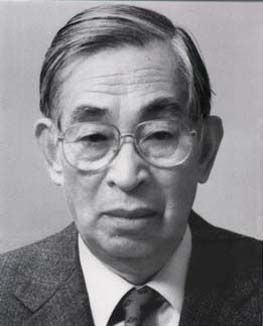
\includegraphics[scale=0.3]{fig/ito.jpg}\\
Kiyosi It\^{o} \\
1915--2008
\end{center}
\end{multicols}
\end{frame}

\begin{frame}{伊藤积分的RS和表达式}
令时间段$[0,T]$中的最长子区间$\|\Pi\|=\max|t_{i+1}-t_{i}|$长度趋于零时,伊藤积分可以写成如下的黎曼-斯蒂尔切斯和的表达式:
\begin{equation*}
I(T)=\int^T_0 g(u)\dif W(u)=\lim_{\substack{\|\Pi\|\to 0 \\ n\to\infty}}\sum^{n-1}_{i=0}g\left(t_i\right)\big[W(t_{i+1})-W(t_{i})\big]
\end{equation*}

\begin{block}{注意:}
不同于确定性积分,以伊藤积分为代表的随机积分,由于是针对布朗运动进行积分求解,因而求算的结果仍然是随机变量。因此,对随机积分的研究不可避免地要涉及对积分的期望、方差等数字特征的求解和计算。
\end{block}
\end{frame}

\begin{frame}{伊藤积分的微分形式}
$$I(T)=\int^T_0 g(t)\dif W(t)$$
上式的伊藤积分还可以写成如下的微分形式(differential form):
\begin{equation*}
\dif I(t)=g(t)\dif W(t)
\end{equation*}
\end{frame}

\begin{frame}{斯特拉托诺维奇积分}
\begin{multicols}{2}
如果选取时间段的中点,则由此构成的随机积分称作斯特拉托诺维奇积分(Stratonovich integral),为了与伊藤积分加以区分,记作:
\[SI(T)=\int^T_0 g(u)\circ \dif W(u) \]

\begin{center}
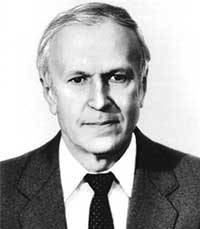
\includegraphics[scale=.5]{fig/Stratonovich.jpg}\\
Ruslan L. Stratonovich\\
1930--1997
\end{center}

\end{multicols}
\end{frame}

\section{伊藤积分的性质}
\begin{frame}{伊藤积分的性质}
假设$g(t), \; t\in[0,T]$是满足平方可积条件\footnote{平方可积条件,就是随机过程$g(t)$的平方之积分是有限的,即:$$\E\int^t_0 g^2(t)\dif t<\infty$$},并且$\mathcal{F}(t)$可测的随机过程。 对于形如$I(t)=\int^t_0 g(u)\dif W(u)$的伊藤积分,其具有如下性质:
\begin{itemize}
	\item 鞅性:$I(t)$是鞅
	\item 期望:$\E[I(t)]=0,\qquad 0\le t\le T$
\end{itemize}
\end{frame}

\begin{frame}{伊藤积分$I(t)=\int^t_0 g(u)\dif W(u)$的性质(cont.)}
\begin{itemize}
	\item 伊藤等距(It\^{o} isometry)
	\begin{equation*}
	\E [I^2(t)]=\E\int^t_0 g^2(u)\dif u
	\end{equation*}
相应地:
\begin{equation*}
\Var[I(t)]=\E[I^2(t)]-[\E I(t)]^2=\E[I^2(t)]=\E\int^t_0 g^2(u)\dif u
\end{equation*}
\item 伊藤积分的二次变差
	\begin{equation*}
	\langle I,I\rangle (t)= \int^t_0 g^2(u)\dif u
	\end{equation*}

\end{itemize}
\end{frame}

\begin{frame}{伊藤积分的性质(cont.)}
\normalsize
与确定性积分类似,伊藤积分具有如下相似的性质:
\begin{enumerate}
\item 可加性(additive):对于两个过程$X_1(t)$和$X_2(t)$,下面的等式成立
\[\int^b_a X_1(t)\dif W(t)+\int^b_a X_2(t)\dif W(t)=\int^b_a \big[X_1(t)+X_2(t)\big]\dif W(t) \]
\item 积分区间可加性:对于$a<b<c$,下面的等式成立
\[\int^c_a X(t)\dif W(t)=\int^b_a X(t)\dif W(t)+\int^c_b X(t)\dif W(t) \]
\item 标量乘法(scalar multiplication)成立:对于任意常数$k$,下面的等式成立
\[\int^b_a kX(t)\dif W(t)=k\int^b_a X(t)\dif W(t) \]
\end{enumerate}
\end{frame}

\begin{frame}{确定性函数伊藤积分之伊藤等距}
假设$W(s)$是一个布朗运动;$f(s)$是关于时间$s$的{\color{red}确定性函数}。则确定性函数(deterministic function)伊藤积分$I(t)=\int^t_0 f(s)\dif W(s)$
具有以下性质:
\[	\E [I^2(t)]=\int^t_0 f^{\,2}(s)\dif s\]
\end{frame}

\begin{frame}{确定性函数伊藤积分的性质}
假设$W(s)$是一个布朗运动;$f(s)$是关于时间$s$的{\color{red}确定性函数}。定义如下伊藤积分:
\begin{equation*}
I(t)=\int^t_0 f(s)\dif W(s)
\end{equation*}
对任意$t\ge 0$,随机变量$I(t)$服从均值为零,方差为$\int^t_0 f^{\,2}(s)\dif s$的正态分布,即:
\begin{equation*}
I(t)\sim \mathcal{N}\left(0, \int^t_0 f^{\,2}(s)\dif s\right)
\end{equation*}

\begin{block}{}
\color{blue}只有在被积函数$f(s)$是确定性的情况下,该结论才成立。如果$f(s)$包含随机项,该结论是不成立的。
\end{block}
\end{frame}


\section{伊藤引理}

\subsection{伊藤过程}

\begin{frame}{伊藤过程的概念}
对于随机过程$\{X(t)\}$,若其满足随机微分方程
\begin{equation*}
\dif X(t)=F(t)\dif t+G(t)\dif W(t)
\end{equation*}
则称作伊藤过程(It\^{o} process)。其中$F(t)$和$G(t)$均是$\mathcal{F}(t)$可测的随机过程。

\begin{block}{}
随机过程$\{X(t)\}$的瞬时增量受到两方面因素的影响:一个是确定性因素的影响,以随机过程$\{F(t)\}$随时间的变化来刻画;另一个是随机性因素的影响,以随机过程$\{G(t)\}$随布朗运动的变化来刻画。
\end{block}
\end{frame}

\begin{frame}{伊藤过程$\dif X(t)=F(t)\dif t+G(t)\dif W(t)$}
假设$F(t)=\mu$,$G(t)=\sigma$,其中$\mu$和$\sigma$均是常数,则由此得到的随机微分方程
$\dif X(t)=\mu\dif t+\sigma\dif W(t)$
就是带有漂移的布朗运动(Brownian motion with drift)。

如果$\mu=0,\; \sigma=1$,则
$\dif X(t)=\dif W(t)$,此时$X(t)$就是标准布朗运动(standard Brownian motion)。

伊藤过程也可以写成对应的积分形式。对于$[0,T]$上的伊藤过程,其积分形式如下:
\begin{equation*}
\int^T_0 \dif X(t)=\int^T_0 F(t)\dif t+\int^T_0 G(t)\dif W(t)
\end{equation*}
{\color{red}积分形式更正式且严谨,而微分形式则相对容易理解。}
\end{frame}

\subsection{伊藤引理}
\begin{frame}{伊藤引理的重要意义}
伊藤引理是随机微积分的核心,其地位相当于普通微积分中的微分理论。

仍需强调的是,由于布朗运动的二次变差不为零,因此随机微分理论具有全新的特征。
\begin{center}
\begin{tabular}{cc}
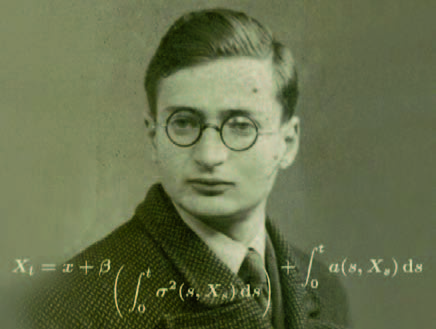
\includegraphics[height=.3\textheight]{fig/doeblin.jpg}& 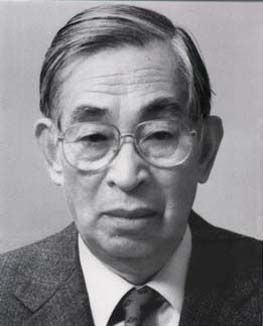
\includegraphics[height=.3\textheight]{fig/ito.jpg}\\
Wolfgang Doeblin& Kiyoshi It\^{o}\\
1915--1940 & 1915--2008
\end{tabular}
\end{center}
\end{frame}

\begin{frame}{回顾:普通微积分的链式法则}
对于一个光滑的函数$G(t)$而言,若有一个可微的函数$f(x)$,根据普通微积分的链式法则(chain rule),我们有:
\[\frac{\dif f\big[G(t)\big]}{\dif t}=f\,'\big[G(t)\big]G'(t) \]
上式也可以写成对应的微分形式:
\begin{equation*}
    \dif f\big[G(t)\big]=f\,'\big[G(t)\big]G'(t)\dif t=f\,'\big[G(t)\big] \dif G(t)
\end{equation*}
\end{frame}


\begin{frame}{回顾:泰勒展开式}
根据泰勒展开式,更精确的形式如下:
\begin{equation*}
    \begin{split}
    \dif f\big[G(t)\big]&=f\,'\big[G(t)\big] \dif G(t)+\frac{1}{2!}f\,''\big[G(t)\big] [\dif G(t)]^2\\
    &\quad +\frac{1}{3!}f^{(3)}\big[G(t)\big] [\dif G(t)]^3+\cdots
\end{split}
\end{equation*}
由于$G(t)$是光滑函数,因此其高阶变差均等于零,即:
\[[\dif G(t)]^2=[\dif G(t)]^3=\cdots=0\]
因此,对于光滑函数$G(t)$,$\dif f\big[G(t)\big]=f\;'\big[G(t)\big]G'(t)\dif t=f\;'\big[G(t)\big] \dif G(t)$已经足以用来刻画$f\big[G(t)\big]$的微分。
\end{frame}

\begin{frame}{$\dif f\big[W(t)\big]$的求解}
由于布朗运动$W(t)$的二次变差不为零。考虑到这一因素,我们就需要使用泰勒展开式,具体如下:
\begin{equation*}
\begin{split}
\dif f\big[W(t)\big]&=f\;'\big[W(t)\big] \dif W(t)+\frac{1}{2}f\;''\big[W(t)\big] [\dif W(t)]^2\\
&=f\;'\big[W(t)\big] \dif W(t)+\frac{1}{2}f\;''\big[W(t)\big] \dif t
\end{split}
\end{equation*}
更高阶的变差均为零,因此泰勒展开式后面的各项均不再体现。
\end{frame}

\begin{frame}{伊藤引理(一维)}\normalsize
定义过程$Z(t)=f(t,X(t))$,并且$X(t)$是满足如下形式的伊藤过程
\[\dif X(t)=F(t)\dif t+G(t)\dif W(t)\]
则随机过程$\{Z(t)\}$满足如下形式的随机微分方程(stochastic differential equation, SDE)
\begin{equation*}
\begin{split}
\dif f(t,X)&=\left[\frac{\partial f(t,X)}{\partial t}+F(t) \frac{\partial f(t,X)}{\partial X}+\frac{1}{2}G^2(t) \frac{\partial^2 f(t,X)}{\partial X^2}\right]\dif t\\
&\qquad +G(t) \frac{\partial f(t,X)}{\partial X} \dif W(t)
\end{split}
\end{equation*}
该方程称作伊藤引理(It\^{o}'s lemma),也称为伊藤公式(It\^{o}'s formula)或伊藤-德布林公式(It\^{o}-Doeblin formula)。
\end{frame}

\begin{frame}{伊藤引理(cont.)}
伊藤引理也可以简写如下:
\begin{equation*}
\dif f(t,X)=\left[f_t+F(t) f_X+\frac{1}{2}G^2(t) f_{XX}\right]\dif t+G(t) f_X \dif W(t)
\end{equation*}
通过伊藤引理,我们可以将随机过程$X(t)$的随机微分方程,通过变量替换的方式转变为随机过程$Z(t)=f[t,X(t)]$的随机微分方程。

\end{frame}

\begin{frame}{布朗运动变化量的乘法法则(product rule)表}
\begin{center}
\begin{tabular}{c|ccc}
\hline & $\dif t$& $\dif W_1(t)$ & $\dif W_2(t)$ \\
\hline
$\dif t$   &    0&0&0\\
$\dif W_1(t)$&0&$\dif t$&$\rho \dif t$\\
$\dif W_2(t)$&0&$\rho \dif t$&$\dif t$\\
\hline
\end{tabular}
\end{center}
其中:$W_1(t)$和$W_2(t)$均是标准布朗运动,并且两者的相关系数为$\rho$。
\end{frame}

\begin{frame}{例1}
已知$\mathcal{F}(t)$可测的随机过程$X(t)$的表达式如下:
\[X(t)=\exp\left[\theta W(t) -\frac{1}{2}\theta^2 t\right] \]
其中:$W(t)$是标准布朗运动,$\theta$是常数。

求$X(t)$的随机微分方程。
\end{frame}

\begin{frame}{例1:解法一}
    根据题意,可得:
    \[Y(t)=\theta W(t) -\frac{1}{2}\theta^2 t,\qquad X[Y(t)]=\exp[Y(t)] \]
    根据伊藤引理,可得:
    \[\begin{split}
    \dif X[Y(t)]&= X_t \dif t+X_Y \dif Y(t)+\frac{1}{2}X_{YY}[\dif Y(t)]^2\\
    &=X(t)\left[\theta \dif W(t) -\frac{1}{2}\theta^2 \dif t\right]+\frac{1}{2}X(t)\left[\theta \dif W(t) -\frac{1}{2}\theta^2 \dif t\right]^2\\
    &=X(t)\theta \dif W(t) -\frac{1}{2}X(t)\theta^2 \dif t+\frac{1}{2}X(t)\theta^2 \dif t\\
    &=\theta X(t)\dif W(t) 
    \end{split} \]
    因此:$\dif X(t)=\theta X(t)\dif W(t) $
\end{frame}

\begin{frame}{例1:解法二}
    根据泰勒展开式进行计算,那么过程如下:
    \[\begin{split}
    \dif X(t)&= X_t \dif t+X_W \dif W(t)+\frac{1}{2}X_{WW}[\dif W(t)]^2\\
    &=-\frac{1}{2}X(t)\theta^2 \dif t+ \theta X(t)\dif W(t)+\frac{1}{2}X(t) \theta^2 \dif t\\
    &=\theta X(t)\dif W(t)
    \end{split} \]

    \begin{block}{说明:}
        第一种方法是针对$X[Y(t)]$进行求偏导的计算,相应地,$X_t[Y(t)]=0$;而第二种方法则是针对$X[t,W(t)]$进行求偏导的计算,相应地,$X_t[t,W(t)]=-\dfrac{1}{2}\theta^2 X(t)$。
    \end{block}
\end{frame}




\begin{frame}{例2}
已知$\mathcal{F}(t)$可测的随机过程$X(t)$的表达式如下:
\[X(t)=W^2(t) \]
其中:$W(t)$是标准布朗运动。

求$X(t)$的随机微分方程。

\begin{block}{}
    使用泰勒展开式,可得:
\[\begin{split}
\dif X&=X_t \dif t+X_W \dif W(t)+\frac{1}{2}X_{WW}[\dif W(t)]^2\\
&=0+2W(t)\dif W(t)+\frac{1}{2}\times 2\dif t\\
&=2W(t)\dif W(t)+\dif t
\end{split} \]
\end{block}
\end{frame}

\begin{frame}{例3}
已知$\mathcal{F}(t)$可测的随机过程$f(S(t))=\ln S(t)$,其中$S(t)$的随机微分方程如下:
\[\dif S(t)=\mu S(t)\dif t+\sigma S(t) \dif W(t) \]
其中:$W(t)$是标准布朗运动,$\mu$和$\sigma$均是常数。

求$f[S(t)]$的随机微分方程。
\end{frame}

\begin{frame}{例3解答}\small
    令$\mu(t)=\mu S(t)$,$\sigma(t)=\sigma S(t) $,根据伊藤引理可得:
    \[\begin{split}
    \dif f&=\left[f_t+\mu(t)f_S+\frac{1}{2}\sigma^2(t)f_{SS}\right]\dif t+\sigma(t) f_S \dif W(t)\\
    &=\left[0+\mu S\frac{1}{S}+\frac{1}{2}\sigma^2 S^2\left(-\frac{1}{S^2} \right)  \right]\dif t+ \sigma S\frac{1}{S} \dif W(t)\\
    &=\left(\mu-\frac{1}{2}\sigma^2 \right) \dif t+\sigma \dif W(t)
    \end{split} \]
   这里也可以使用泰勒展开式进行求解,具体如下:
    \[\begin{split}
    \dif f&=f_t\dif t+f_S\dif S+\frac{1}{2}f_{SS}(\dif S)^2\\
    &=0+\frac{1}{S}\mu S\dif t+\sigma S \dif W(t)+\frac{1}{2}\left(-\frac{1}{S^2} \right) (\sigma^2S^2\dif t)\\
    &=\left(\mu-\frac{1}{2}\sigma^2 \right) \dif t+\sigma \dif W(t)
    \end{split} \]
    \end{frame}

\begin{frame}{例4}
假设$f(S,t)=S-Ke^{-r(T-t)}$,并且其中的随机过程$S(t)$的随机微分方程如下:
\[\dif S(t)=\mu S(t)\dif t+\sigma S(t) \dif W(t) \]
其中:$W(t)$是标准布朗运动,$\mu$和$\sigma$均是常数。

求$f(S,t)$的随机微分方程。
\end{frame}

\begin{frame}{例4解答}
    使用泰勒展开式进行求解,具体如下:
\[\begin{split}
\dif f&= f_t \dif t+f_S\dif S+\frac{1}{2}f_{SS}(\dif S)^2\\
&=-K{\rm e}^{-r(T-t)}\cdot r \dif t+\dif S+0\\
&=-rK{\rm e}^{-r(T-t)} \dif t+\mu S\dif t+\sigma S \dif W(t)\\
&=\Big[-rK{\rm e}^{-r(T-t)}+\mu S\Big]\dif t+\sigma S \dif W(t)
\end{split} \]
因此:$$\dif f(S,t)=\Big[-rK{\rm e}^{-r(T-t)}+\mu S(t)\Big]\dif t+\sigma S(t) \dif W(t)$$
\begin{block}{说明:}
    此处的随机微分方程常常用于金融远期合约的建模。
\end{block}

\end{frame}


\begin{frame}{例5}
假设$f(S,t)=Se^{r(T-t)}$,并且其中的随机过程$S(t)$的随机微分方程如下:
\[\dif S(t)=\mu S(t)\dif t+\sigma S(t) \dif W(t) \]
其中:$W(t)$是标准布朗运动,$\mu$和$\sigma$均是常数。

求$f(S,t)$的随机微分方程。
\end{frame}

\begin{frame}{例5解答}
    使用泰勒展开式进行求解,具体如下:
    \[\begin{split}
    \dif f&= f_t \dif t+f_S\dif S+\frac{1}{2}f_{SS}(\dif S)^2\\
    &=-S{\rm e}^{r(T-t)}\cdot r \dif t+{\rm e}^{r(T-t)}\dif S+0\\
    &=-rS{\rm e}^{r(T-t)} \dif t+{\rm e}^{r(T-t)}[\mu S\dif t+\sigma S \dif W(t)]\\
    &={\rm e}^{r(T-t)}\Big[\big(-rS+\mu S\big)\dif t+\sigma S \dif W(t)\Big]\\
    &=S{\rm e}^{r(T-t)}[(\mu-r)\dif t+ \sigma \dif W(t)]\\
    &=f(S,t)[(\mu-r)\dif t+ \sigma \dif W(t)]
    \end{split} \]
\begin{block}{说明:}
此处的随机微分方程常常用于金融期货合约的建模。
\end{block}

    \end{frame}


\begin{frame}{二维伊藤引理}
令函数$f(t,x,y)$的各一阶和二阶偏导数均存在且连续。假设$X(t)$和$Y(t)$均是伊藤过程,则相应的二维伊藤公式如下:
\begin{equation*}
\begin{split}
df&=f_t \dif t+f_x\dif X(t)+f_y\dif Y(t)+f_{xy}[\dif X(t)\dif Y(t)]\\
&\quad +\frac{1}{2}f_{xx}[\dif X(t)]^2+\frac{1}{2}f_{yy}[\dif Y(t)]^2
\end{split}
\end{equation*}
\end{frame}

\begin{frame}{伊藤乘法法则}
假设$X(t)$和$Y(t)$均是伊藤过程,则有:
\begin{equation*}
\dif \Big[X(t)Y(t)\Big]=X(t)\dif Y(t)+Y(t)\dif X(t)+{\color{red}\dif X(t)\dif Y(t)}
\end{equation*}

\begin{block}{注意:}
对于普通的函数$F(t)$和$G(t)$,其微分的乘法法则如下:
\[\dif\Big[F(t)G(t)\Big]=F(t)\dif G(t)+G(t)\dif F(t) \]
相比之下,在伊藤过程中,其微分的乘法却多出一项$\dif X(t)\dif Y(t)$,称为交叉变差项(cross variation term)
,出现这项的原因在于:布朗运动的二次变差不为零。
\end{block}
\end{frame}

\begin{frame}{伊藤乘法法则(cont.)}
\normalsize
对$\dif \Big[X(t)Y(t)\Big]=X(t)\dif Y(t)+Y(t)\dif X(t)+{\dif X(t)\dif Y(t)}$的两侧同时取积分,可得:
\begin{align*}
\int^t_0 \dif \Big[X(u)Y(u)\Big]&=\int^t_0 X(u)\dif Y(u)+\int^t_0 Y(u)\dif X(u) +\int^t_0 \dif\langle X, Y\rangle(u)\\
X(t)Y(t)&=X(0)Y(0)+\int^t_0 X(u)\dif Y(u)+\int^t_0 Y(u)\dif X(u)\\
&\qquad +\int^t_0 \dif\langle X, Y\rangle(u)
\end{align*}
其中:$\dif\langle X, Y\rangle(u)=\dif X(u)\dif Y(u)$,也就是交叉变差项。
\end{frame}

\begin{frame}{伊藤乘法法则的推论}
假设$X(t)$是伊藤过程,$G(t)$是确定性函数,则有:
\begin{equation*}
\dif \Big[X(t)G(t)\Big]=X(t)\dif G(t)+G(t)\dif X(t)
\end{equation*}

\begin{block}{注意:}
此处没有了交叉变差项$\dif G(t)\dif X(t)$,这是因为确定性函数$G(t)$当中不包含随机项,因此将之与随机函数$X(t)$求交叉变差后,$\dif G(t)\dif X(t)\equiv 0$,自然可以将之忽略。
\end{block}
\end{frame}

\begin{frame}{伊藤乘法法则的推论(cont.)}\normalsize
对$\dif \Big[X(t)G(t)\Big]=X(t)\dif G(t)+G(t)\dif X(t)$的两侧同时取积分,可得:
\begin{align*}
\int^t_0 \dif \Big[X(u)G(u)\Big]&=\int^t_0 X(u)\dif G(u)+\int^t_0 G(u)\dif X(u)\\
X(t)G(t)&=X(0)G(0)+\int^t_0 X(u)\dif G(u)+\int^t_0 G(u)\dif X(u)\label{int-part}
\end{align*}
进一步可以得到:
\begin{align*}
\int^t_0 X(u)\dif G(u)&=X(u)G(u)\Big|^t_0-\int^t_0 G(u)\dif X(u)\\
\int^t_0 G(u)\dif X(u)&=X(u)G(u)\Big|^t_0-\int^t_0 X(u)\dif G(u)
\end{align*}
此处的结果,与普通积分中的分部积分非常相似。
\end{frame}

\begin{frame}{例6}
假设随机过程$X(t)$对应的随机微分方程如下:
\[\dif X(t)=-\frac{1}{2}bX(t)\dif t+\frac{1}{2}\sigma \dif W(t) \]
求$Y(t)=X(t)\exp\qty(\displaystyle\frac{1}{2}bt)$的随机微分方程。
\end{frame}


\begin{frame}{例6解答}
    注意到$Y(t)$是由确定性函数$G(t)=\exp\qty(\displaystyle\frac{1}{2}bt)$与随机函数$X(t)$所构成的。因此:
    \[\begin{split}
    \dif Y(t)&= X(t)\dif G(t)+G(t)\dif X(t)\\
    &=X(t)\cdot \frac{1}{2}b\exp\qty(\displaystyle\frac{1}{2}bt)\dif t+\exp\qty(\displaystyle\frac{1}{2}bt)\left[-\frac{1}{2}bX(t)\dif t+\frac{1}{2}\sigma \dif W(t)\right]\\
    &=\frac{1}{2}\sigma \exp\qty(\displaystyle\frac{1}{2}bt)  \dif W(t)
    \end{split} \]
    
    \end{frame}


\begin{frame}{例7}
已知关于$S(t)$的随机微分方程如下:
\[\dif S(t)=\mu S(t)\dif t +\sqrt{V(t)}S(t)\dif W_1(t) \]
其中:
\[\dif V(t)=[a+b V(t)]\dif t +\xi V(t)^{\alpha}\dif W_2(t) \]
并且$W_1(t)$和$W_2(t)$均是标准布朗运动,两者的相关系数为$\rho$。

求$f(t,S,V)$的随机微分方程。
\end{frame}


    \begin{frame}{例7解答}
        根据伊藤乘法法则可得:$$[\dif W_1(t)]^2=[\dif W_2(t)]^2=\dif t,\quad [\dif W_1(t)\dif W_2(t)]=\rho\dif t$$
        由泰勒展开式可得:
        \[\dif f(t,S,V)=f_t\dif t+f_S\dif S+f_V\dif V+f_{SV}\dif S\dif V+\frac{1}{2}\left[f_{SS}(\dif S)^2+f_{VV}(\dif V)^2\right]\]
        由于:
        \[    (\dif S)^2=VS\dif t\qquad 
        (\dif V)^2=\xi^2 V^{2\alpha}\dif t\]
        \[\dif S\dif V=\sqrt{V}S\xi V^{\alpha}\rho\dif t=\rho\xi SV^{\alpha+0.5}\dif t
    \]
\end{frame}


\begin{frame}{例7解答(cont.)}
        因此:
        \[\begin{split}
        \dif f&=f_t\dif t+f_S\left(\mu S\dif t +\sqrt{V}S\dif W_1\right)+f_V[(a+b V)\dif t +\xi V^{\alpha}\dif W_2]\\
        &\quad +f_{SV}\left(\rho\xi SV^{\alpha+0.5}\dif t\right)+\frac{1}{2}\left(f_{SS}VS\dif t+f_{VV}\xi^2 V^{2\alpha}\dif t\right)\\
        &=\left[f_t+\mu S f_S+(a+bV)f_V+\rho\xi SV^{\alpha+0.5}f_{SV}+\frac{1}{2}SVf_{SS}+\frac{1}{2}\xi^2 V^{2\alpha}f_{VV} \right]\dif t \\
        &\quad +\sqrt{V}Sf_S \dif W_1+\xi V^{\alpha}f_V\dif W_2
        \end{split} \]

        \begin{block}{说明:}
            上面的随机过程包含两个部分:一个是资产价格的过程,另一个是相应波
动率的过程。该模型也因此被称为随机波动率模型(stochastic volatility model),由
史蒂文·赫斯顿(Steven Heston)于1993年提出。
        \end{block}
\end{frame}


\begin{frame}{例8}
    已知$W(t)$是标准布朗运动,证明:
\[\int^t_0 W^2(s)\dif W(s)=\frac{1}{3}W^3(t)-\int^t_0 W(s)\dif s \]

\begin{block}{思路}
    以$\frac{1}{3}W^3(t)$为突破口,利用伊藤引理。
\end{block}
\end{frame}


\begin{frame}{例8解答}\small
        假设$X(t)=\displaystyle\frac{1}{3}W^3(t)$,根据伊藤引理可得:
        \[\dif X=X_t \dif t+X_W\dif W+\frac{1}{2}X_{WW}(\dif W)^2=0+W^2\dif W+W\dif t \]
        因此:
        \[\dif X(t)=W^2(t)\dif W(t)+W(t)\dif t \]
        对上式的两端取积分,可得:
        \[\begin{split}
        \int^t_0\dif X(s)&=\int^t_0W^2(s)\dif W(s)+\int^t_0 W(s)\dif s\\
        \int^t_0W^2(s)\dif W(s)&=\int^t_0\dif X(s)-\int^t_0 W(s)\dif s\\
        &=X(t)-X(0)-\int^t_0 W(s)\dif s\\
        &=\frac{1}{3}W^3(t)-\frac{1}{3}W^3(0)-\int^t_0 W(s)\dif s\\
        \end{split} \]
    \end{frame}


    \begin{frame}{例8解答(cont.)}
        因此:
        \[\int^t_0W^2(s)\dif W(s)=\frac{1}{3}W^3(t)-\int^t_0 W(s)\dif s \]

        \begin{block}{注意:}
            对于确定性函数$f(t)$,若$f(0)=0$,则其积分的结果如下:
            \[\int^t_0 f^{\;2}(s)\dif f(s)=\left.\frac{1}{3}f^{\;3}(s)\right|^t_0=\frac{1}{3}f^{\;3}(t)-\frac{1}{3}f^{\;3}(0)=\frac{1}{3}f^{\;3}(t) \]
            而本题对于布朗运动所做的随机积分,结果中却多出一项,两者的差异源自布朗运动的二次
变差不为零。
        \end{block}
       
\end{frame}



\end{document}
